\section{The Queue Transmission Model}


%% TODO(fwt): We need to say that we handle expected number of cars instead of
%% physical cars, so its fine to have fractions of cars.

A Queue Transmission Model (QTM) is the tuple $(\Qset, \Lset, \vecDT, \MatQIN)$,
where \Qset and \Lset are, respectively, the set of queues and set of lights;
%
\vecDT is a vector of size \Nn representing the discretization in intervals of
the simulation horizon $[0,\TMAX]$ and the duration \remark{in seconds} of the
$n$-th time interval is denoted as \DT[n];
%
%%
%% TODO(fwt): Maybe mention that car that are denied entry could be stored in a
%% infinity capacity queue and eventually be allowed to enter the network. Also
%% point out that this case doesn't happen in our experiments
%%
%% TODO(fwt): Maybe mention that add \QIN{i} can estimate through a model
%% learned from historical data.
%
and \MatQIN is a matrix $|\Qset| \times \TMAX$ in which \QIN{i,n} represents the
flow of cars \remark{trying} to enter queue $i$ from the outside of the network
at time $n$.



A \textbf{traffic light} $\tl \in \Lset$ is defined as the tuple~$(\CTMIN{\tl},
\CTMAX{\tl}, \Pset_\tl, \VecPTMIN{\tl}, \VecPTMAX{\tl})$, where:

\begin{itemize}
%
\item $\Pset_\tl$ is the set of phases of $\tl$;
%
\item \CTMIN{\tl} (\CTMAX{\tl}) is the minimum (maximum) allowed cycle time for
  \tl; and
%
\item \VecPTMIN{\tl} (\VecPTMAX{\tl}) is a vector of size $|\Pset_\tl|$ and
  \PTMIN{\tl}{k} (\PTMAX{\tl}{k}) is the minimum (maximum) allowed time for
  phase $k \in \Pset_\tl$. 
%
\end{itemize}


A \textbf{queue} $i \in \Qset$ represents a segment of road that vehicles
traverse at free flow speed; once traversed, the vehicles are vertically stacked
in a stop line queue.
% of maximum capacity \QMAX{i}.
%
Formally, a queue~$i$ is defined by the tuple~$(\QMAX{i}, \QDELAY{i}, \QOUT{i},
\Fvec_i, \Prvec_i, \QPset{i})$ where:

\begin{itemize}
%
%% TODO(fwt): clarify that this is the capacity of stop line queue
\item \QMAX{i} is the maximum capacity of $i$;
%
\item \QDELAY{i} is the time required to traverse $i$ and reach the stop line;
%
\item \QOUT{i} represents the maximum traffic flow from $i$ to the outside of the
modeled network;
%
\item $\Fvec_i$ and $\Prvec_i$ are vectors of size \Qn and their $j$-th entry
  (i.e., \FMAX{i}{j} and \FTURN{i}{j}) represent the maximum flow from queue $i$
  to $j$ and the turn probability from $i$ to $j$ ($\sum_{j \in
  \Qset}\FTURN{i}{j} = 1$), respectively; and
%
\item \QPset{i} denotes the set of traffic light phases controlling
\remark{the outflow of} queue $i$.
%
\end{itemize}


Differently than CTM \cite{daganzo1994cell,lin2004enhanced}, QTM does not assume
that \remark{$\DT[n] = \QDELAY{i}$} for all $n \in \{1,\dots,\Nn\}$, that is,
the QTM can represent non-homogeneous time intervals.
%
The only requirement over \DT[n] is that no traffic light maximum phase time is
smaller than any \DT[n] since we are only allowed to change phases between time
intervals; formally, $\DT[n] \le \min_{\tl \in \Lset, k \in \Pset_\tl}
\PTMAX{\tl}{k}$ for all $n \in \{0,\dots,\Nn\}$.


\remark{FWT: either bring forward a small network and explain it here or don't
mention ``\cref{fig:network3,fig:network6,fig:network9}''}




\subsection{Traffic Flow Simulation with QTM}

In this section, we present how to simulate traffic flow in a network using QTM
and non-homogeneous time intervals \DT[].
%
We assume for the remainder of this section that a \emph{valid} control plan for
all traffic lights is fixed and given as parameter;
%
formally, for all $\tl \in \Lset$, $k \in \Pset_\tl$, and interval $n \in
\{0,\dots,N\}$, the binary variable $\p{\tl}{k}$ is known a priori and indicates
if phase $k$ of light \tl is active~(i.e., $\p{\tl}{k} = 1$) or not on interval
$n$.


We represent the problem of finding the flow between queues as a linear program
(LP) over the following variables defined for all interval $n \in
\{1,\dots,\Nn\}$ and queues $i$ and $j$:

\begin{itemize}
%
\item $\q{i} \in [0,\QMAX{i}]$: traffic volume of queue $i$ during interval $n$
%
\item $\inq{i} \in [0,\QIN{i}{n}]$: inflow to the network via queue $i$
during interval $n$
%
\item $\outq{i} \in [0,\QOUT{i}]$: outflow from the network via queue $i$ during
interval $n$
%
\item $\f{i}{j} \in [0,\FMAX{i}{j}]$: flow from queue $i$ into queue $j$ during
interval $n$
%
\end{itemize}

%% FWT: These constraints are not necessary because we defined the domain of the
%% variables in the paragraph above
%\inq{i} &\le \QIN{i}{n} \tag{C1}\label{eq:C1}\\ 
%\outq{i} &\le \QOUT{i} \tag{C2}\label{eq:C2}\\
% \q{i} &\le \QMAX{i} \tag{C9}\label{eq:C9}\\


%% TODO(fwt): add glue here

The maximum traffic flow from queue $i$ to queue $j$ is enforced by
\cref{c:turnProb,c:maxFlow}.
%
\eqref{c:turnProb} ensures that only the fraction $\FTURN{i}{j}$ of the total
internal outflow of $i$ goes to $j$, and \eqref{c:maxFlow} forces the flow from
$i$ to $j$ to be zero if all phases controlling $i$ are inactive (i.e.,
$\p{\ell}{k} = 0$ for all $k \in \QPset{i}$).
%
If more than one phase $\p{\ell}{k}$ is active, then \eqref{c:maxFlow} is
subsumed by the domain upper bound of $\f{i}{j}$.
%
\begin{cAlign}
\f{i}{j} &\le \FTURN{i}{j} \sum_{k=1}^{\Qn}  \f{i}{k} \tagconstrain{c:turnProb}\\
\f{i}{j} &\le \FMAX{i}{j} \sum_{\p{\ell}{k} \in \QPset{i}} {\p{\ell}{k}}
\tagconstrain{c:maxFlow}
\end{cAlign}


%% TODO(fwt): improve the beginning of this paragraph

To simplify the presentation of remainder of the LP, we define the helper
variables \qin{i}~\eqref{def:qin}, \qout{i}~\eqref{def:qout}, and
\tn[n]~\eqref{def:tn} to represent the volume of traffic to enter and leave
queue $i$ during interval $n$, and the time elapsed since the beginning of the
simulation until the end of interval \DT[n].
%
Using these helper variables, the preservation of flow principle for queue $i$
and \textit{homogeneous} \DT[] is simply $\q{i} = \q[n-1]{i} - \qout[n-1]{i} +
\qin[n-1]{i}$; however, a more sophisticated principle is need for
non-homogeneous time intervals \remark{because \DT[n-1] might be smaller than
\QDELAY{i}, therefore, there are cars at the stop line of $i$ in the beginning
of \DT[n] that started traversing $i$ before \DT[n-1].}
%
\toIain{Triple check my explanation.}
%
\toIain{I removed the constraint $\q{i} \le \frac{\DT[n]}{\DT[m]}\qin[m]{i} -
\qout{i}$ because it seems to be subsumed by \eqref{c:qUpdate}. If they are
needed, add it back with an explanation}
%
%% FWT: Text related to the removed constraint:
%with the constraint \ref{eq:C7} that the total flow out of queue $i$ during
%interval $n$ cannot exceed the sum of the volume of the queue at the start of
%that interval and the volume of traffic arriving at the stop line during the
%interval.
%
\begin{cAlign}
%
\qin{i} &= \DT (\inq{i} + \sum_{j=1}^{\Qn} \f{j}{i}) \tagconstrain{def:qin} \\
%
\qout{i} &= \DT (\outq{i} +  \sum_{j=1}^{\Qn} \f{i}{j})
\tagconstrain{def:qout}\\
%
\tn[n] &= \sum_{x=1}^{n} \DT[x] \tagconstrain{def:tn}
%
\end{cAlign}


In order to account for the \remark{misalignment} of the different \DT[] and
\QDELAY{i}, we need to find the volume of traffic that was able to arrive at
queue $i$, traverse it (i.e., wait \QDELAY{i} seconds), and reach the stop line
before \DT[n] is over.
%
%% TODO(fwt): improve this explanation
%
This volume of traffic is obtained by integrating over the interval\toIain{What
interval?} with the rate at which traffic was arriving during the interval $m$
containing the time $\tn - \QDELAY{i}$ such that $\tn[m] \le \tn-\QDELAY{i} <
\tn[m+1]$.
%
The input rate of queue $i$ during interval $m$ is found by dividing
$\qin[m]{i}$ with $\DT[m]$, and then the total traffic arriving during the
interval $n$ is found by multiplying this rate by $\DT$.
%
The preservation of flow principle for non-homogeneous time steps is presented
in \eqref{c:qUpdate}.
%
\toIain{Explain \cref{eq:C10}}
%
\begin{cAlign}
%
\q{i} &= \q[n-1]{i} - \qout[n-1]{i} + \frac{\DT[n]}{\DT[m]}\qin[m]{i}
\tagconstrain{c:qUpdate}\\
%
\frac{\DT[n]}{\DT[m]}\qin[m]{i}  + \sum \limits_{k=m+1}^n \qin[k]{i} &\le
\QMAX{i} - \q[n-1]{i} \tagconstrain{eq:C10}
%
\end{cAlign}


\remark{Show diagrams with traffic predictions converging as time increment gets smaller.
  Validates that large time-steps are rough approximations while model behavior converges
for small time steps.}

\begin{figure*}[t!]
\centering
%  trim={<left> <lower> <right> <upper>}
\subfigure[]{
\label{subfig:converg_a}
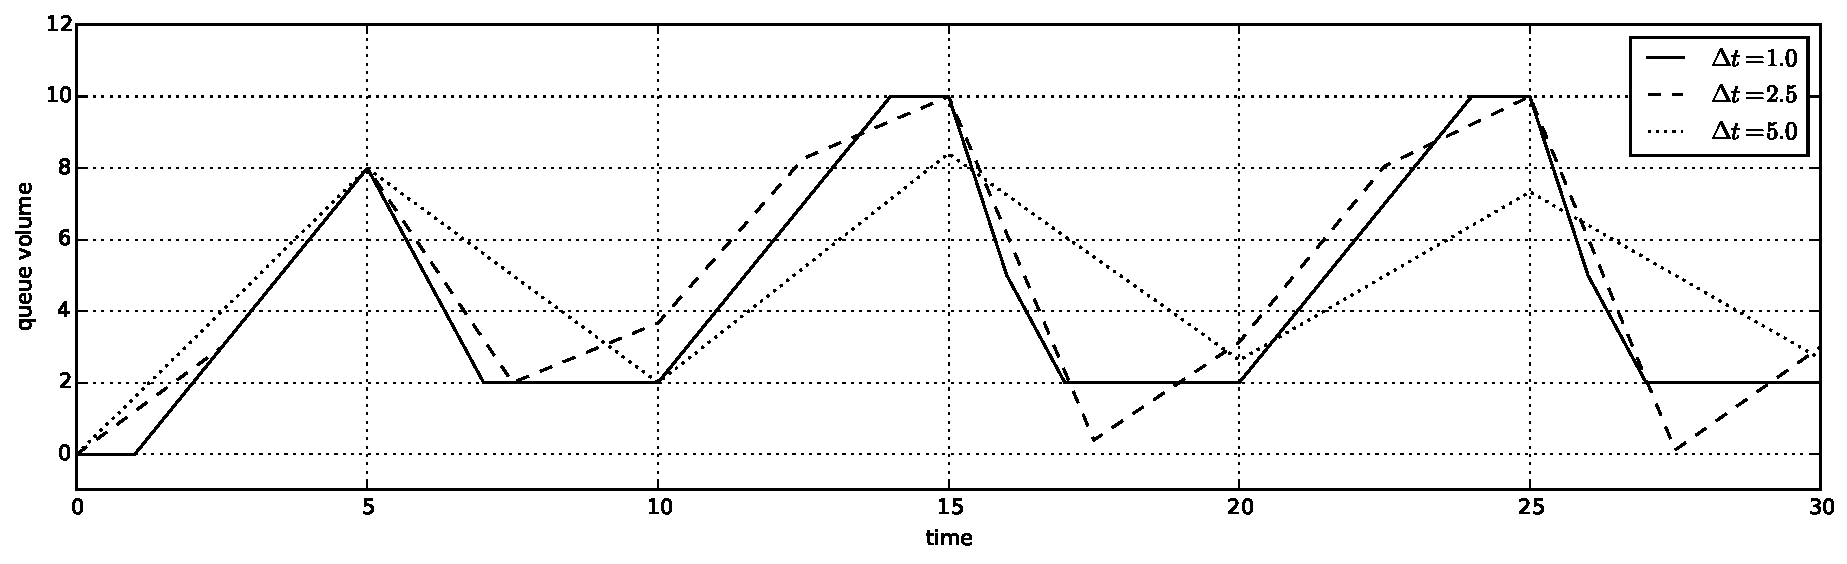
\includegraphics[width=1.0\textwidth,trim={0cm 0cm 0cm 0cm},clip]{convergence.pdf}
}
\subfigure[]{
\label{subfig:converg_b}
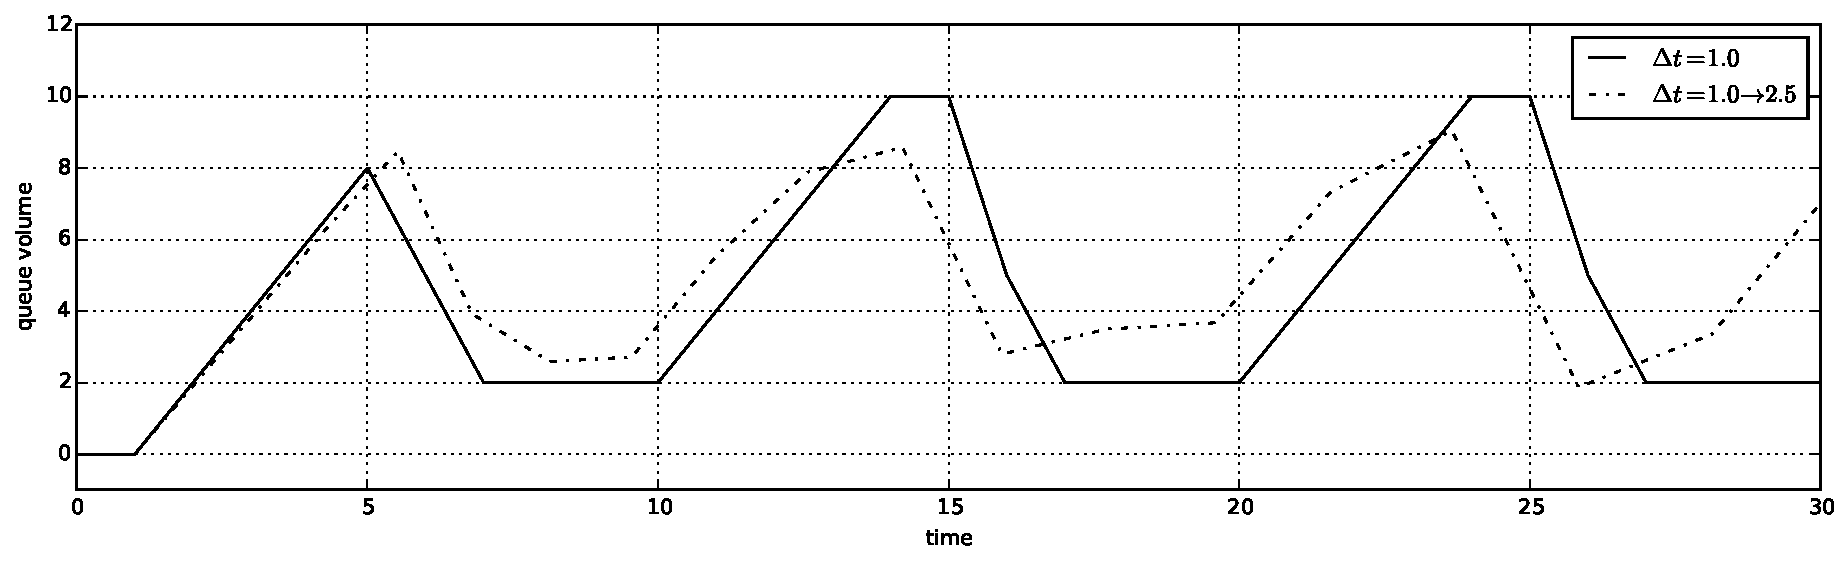
\includegraphics[width=1.0\textwidth,trim={0cm 0cm 0cm 0cm},clip]{convergence_vari.pdf}
}
\caption{An example showing the evolution of traffic volume in a queue over
time. (a) Convergce with increasing refinement of $\Delta t$ from $5.0$ down to
$1.0$. (b) Dilation of $\Delta t$ from $1.0$ to $2.5$ compared to a fixed
$\Delta t$ of $1.0$.}

\end{figure*}

\begin{figure*}[t!]
\centering
%  trim={<left> <lower> <right> <upper>}

\label{subfig:converg_c}
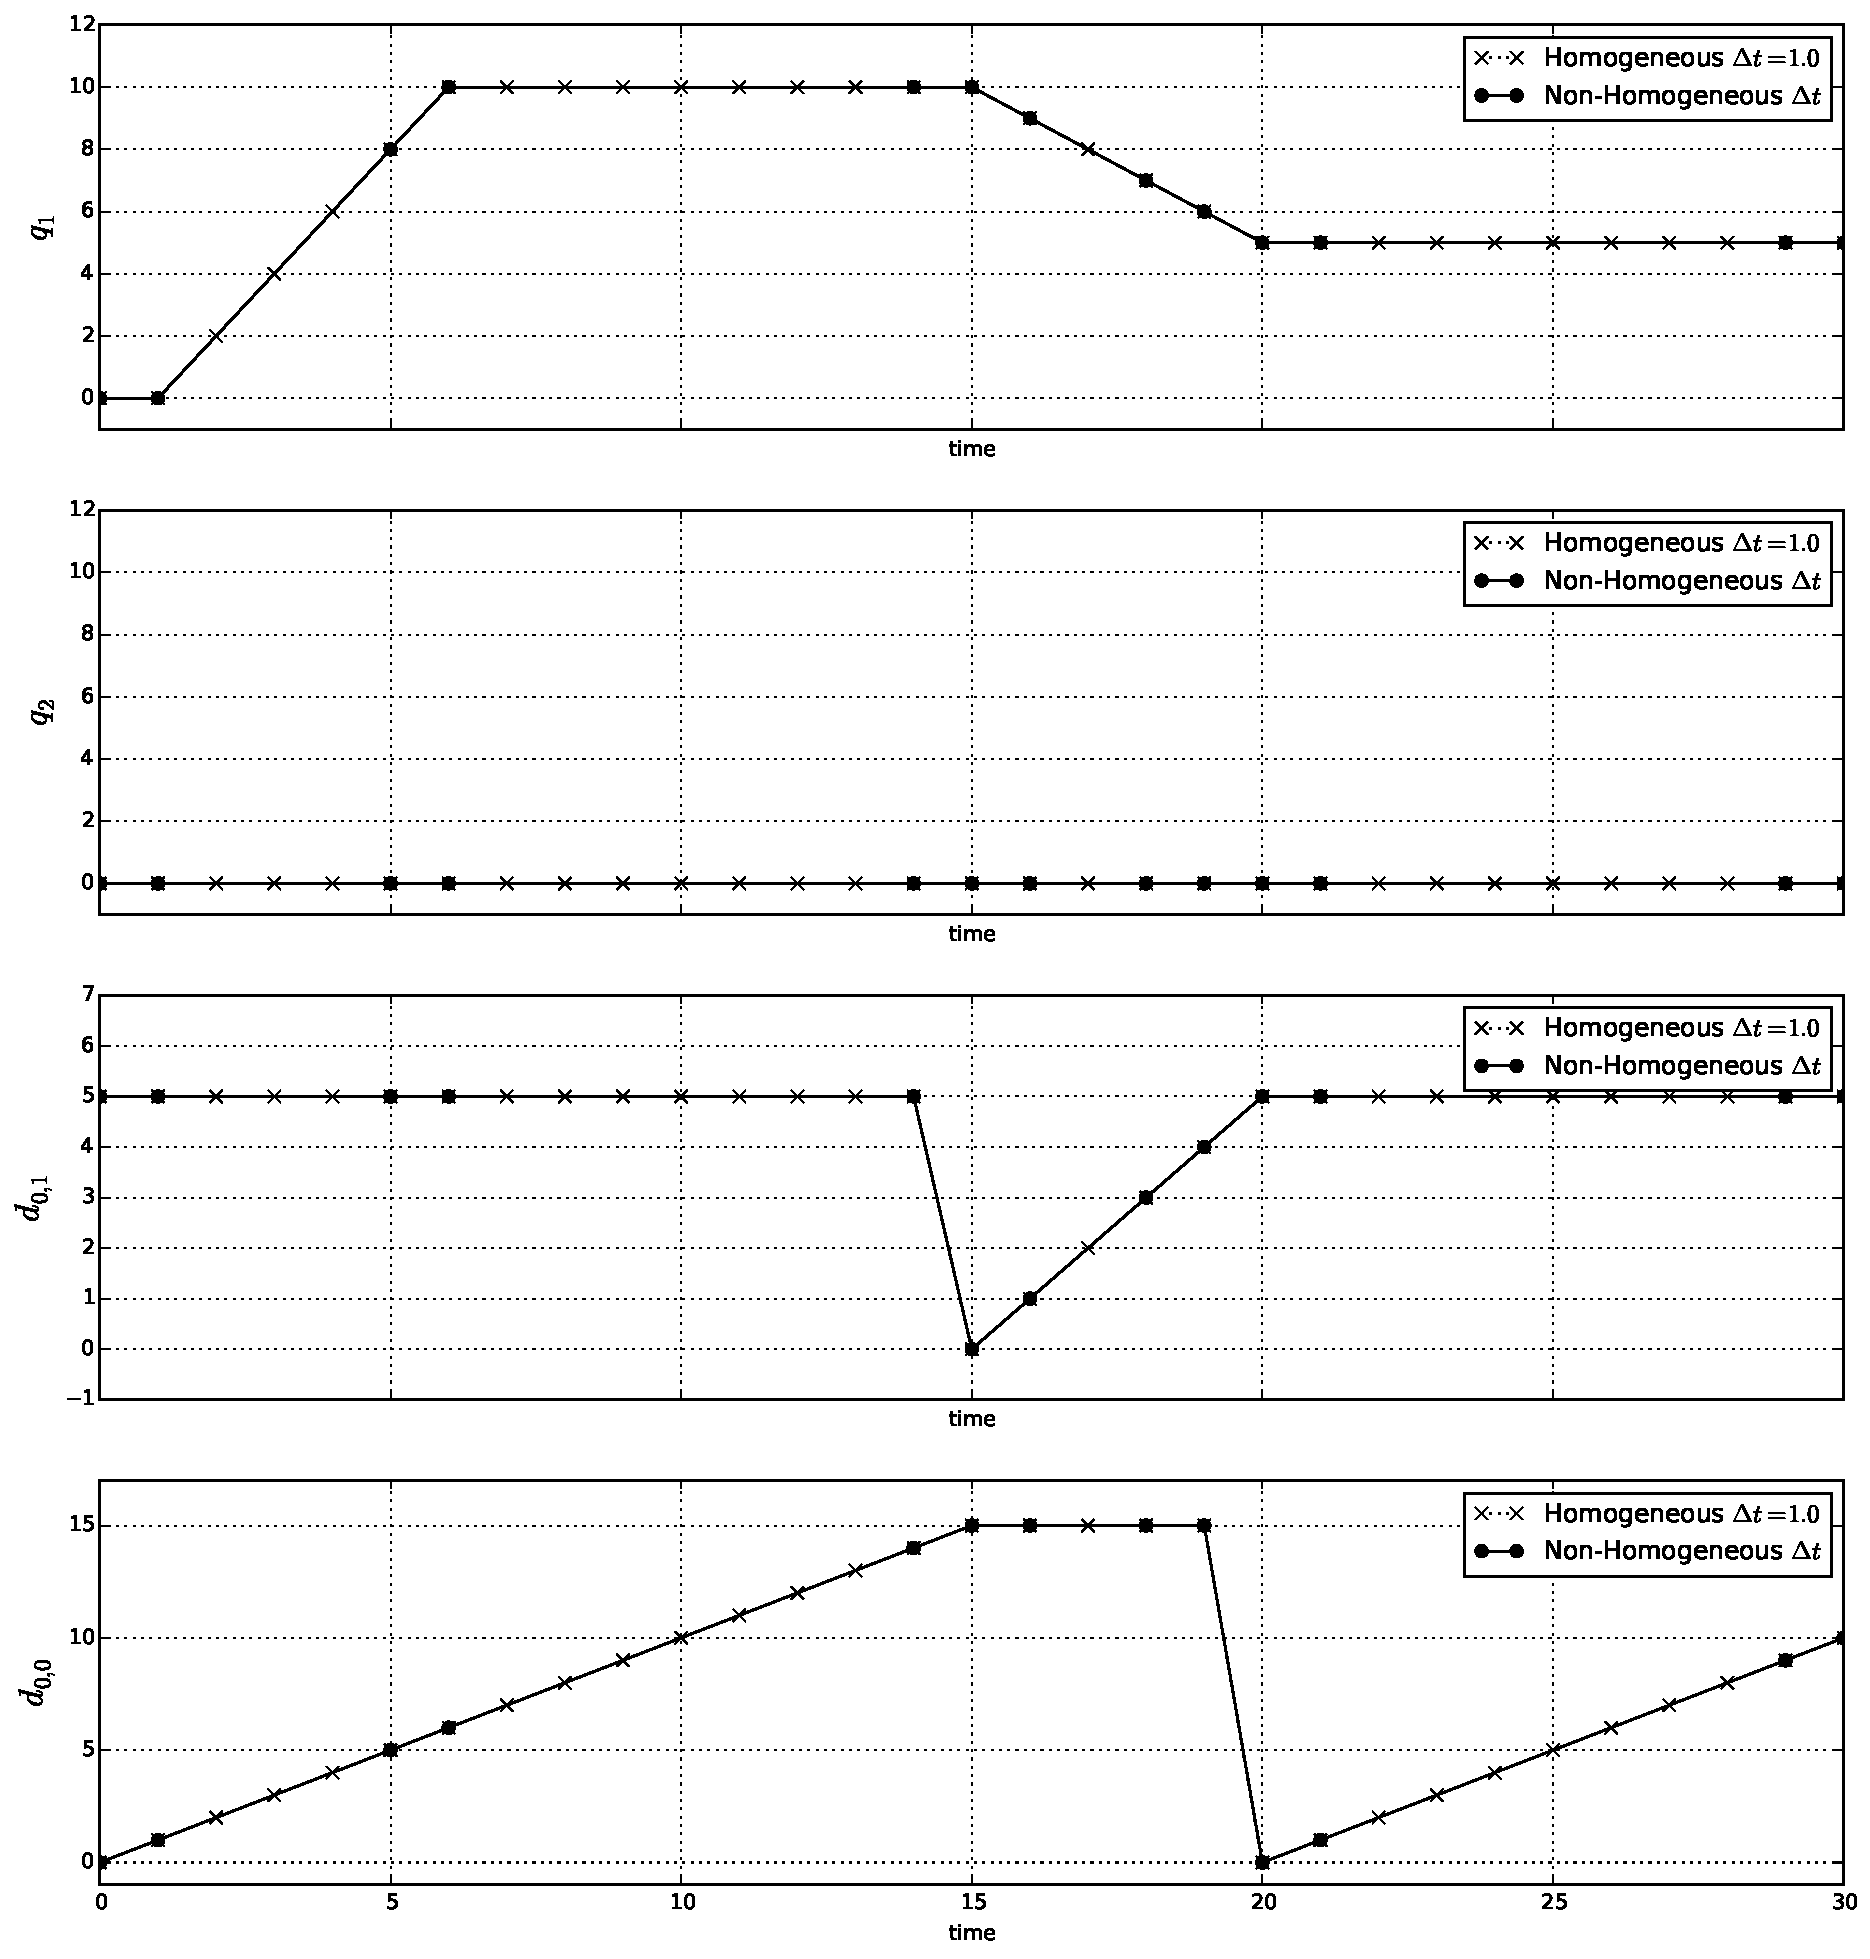
\includegraphics[width=1.0\textwidth,trim={0cm 0cm 0cm 0cm},clip]{convergence_NH.pdf}
\caption{An example showing the convergence between a homogeneous solution with
$\Delta t=1.0$ and a non-homogeneous solution over 30 seconds for the same
network. By using non-homogeneous time steps the same solution is found with
only 14 sample points compared to 30 for homogeneous solution.}

\end{figure*}


\remark{FWT: introduce the objective function, explain its parts and relate to
Lin and Wang}

\trbcite{lin2004enhanced} derive an objective function for the minimisation of
total delay based on the difference between the cumulative departure and arrival
curves at the origin and destination. However, such an approach requires the
network to be cleared at the end of the optimisation period. We derive an
objective function for the maximisation of flow in the network, and apply it to
every queue in the network at $\qout{i}$,


\begin{equation}
\textrm{maximise} \left( \sum\limits_{n=1}^{\Nn} \sum\limits_{i=1}^{\Qn} (\TMAX - \tn + 1) \qout{i} + \sum\limits_{n=1}^{\Nn} \sum\limits_{i=1}^{\Qn} (\TMAX - \tn + 1) \inq{i} \right) 
\tag{O1}\label{eq:O1}
\end{equation}

And with the addition of the second $\inq[]{i}$ term, \ref{eq:O1} also ensures
that \remark{old-C1}, \remark{old-C2}, and \ref{c:maxFlow} are also at their maximum upper
bound.

\remark{It is explanatory here to show the inflow/outflow and delay curves and
explain graphically what is going on and how this objective relates.}

\remark{Finish section conclusion}

Constraints \ref{c:turnProb} to \ref{eq:C10} form a dynamic, piecewise linear model
of flow in the network over time as a \remark{function of $\Pi$}.




\section{Traffic Control with QTM as an MILP}


\remark{Tell goal of this section and remind the reader about \p{\ell}{k}}
%Alternatively we can define $p_j^n$ as a binary
%variable and solve to find both a network flow and an optimal signal plan for a
%given objective function.


\remark{Define: $\pd{\ell}{k}$ -- continuous -- $[0,\PTMAX{\ell}{k}]$ -- duration of
phase $k$ of light $\ell$ during interval $n$}

%\subsubsection{Phase constraints}

First we map each $p_i^n$ to a signal phase $k$ of a light $\ell$ as
$\p{\ell}{k}$ (Note that there could be more than one queue mapped to each
$\p[]{\ell}{k}$, or their could be none). Then we define a set of constraints
for the signal phases. For each traffic light $\ell$, we constrain the phases of
$\ell$ such that exactly one phase is active in each interval $n$, and so that
they activate sequentially,

\begin{align}
\sum\limits_{k=1}^{\Pn} \p{\ell}{k} &= 1\tag{C11}\label{eq:C11}\\
\p{\ell}{k} + \p{\ell}{k+1} &\le 1\tag{C12}\label{eq:C12}\\
\p[n-1]{\ell}{k} &\le \p{\ell}{k} + \p{\ell}{k+1}\tag{C13}\label{eq:C13}
\end{align}

where $k+1=1$ if $k=P_l$. The constraints \ref{eq:C12} and \ref{eq:C13} ensure
that if $\p[]{\ell}{k}$ was active during interval $n-1$ and has become inactive
in interval $n$, then $p_{l,k+1}$ becomes active in interval $n$.

Next we enforce the minimum and maximum phase durations, $\PTMIN{\ell}{k}$ and
$\PTMAX{\ell}{k}$ for each $\p[]{\ell}{k}$, by defining a duration variable
$\pd[]{\ell}{k}$ for each phase. When $\p[]{\ell}{k}$ is active,
$\pd[]{\ell}{k}$ holds the elapsed time since the start of phase $k$, and when
phase $k$ is inactive $\pd{\ell}{k}$ is constant and holds the duration of the
last phase until the next activation,

\begin{equation}
\pd{\ell}{k} = 
\begin{cases}
\pd[n-1]{\ell}{k} + \DT[n-1] & \p[n-1]{\ell}{k}=1,\p{\ell}{k}=1\\
\pd[n-1]{\ell}{k} & \p{\ell}{k}=0\\
0 & \p[n-1]{\ell}{k}=0,\p{\ell}{k}=1
\end{cases}
\end{equation}

We achieve this by applying a set of linear envelope constraints, using the
``big M'' trick to activate each section of the envelope depending on the state
of $\p[]{\ell}{k}$, where ``big M'' can be limited to $\PTMAX{\ell}{k}$.

\begin{align}
\pd{\ell}{k} &\le \pd[n-1]{\ell}{k} + \DT[n-1] \p[n-1]{\ell}{k} + \PTMAX{\ell}{k} (1 - \p[n-1]{\ell}{k})\tag{C14}\label{eq:C14}\\
\pd{\ell}{k} &\ge \pd[n-1]{\ell}{k} + \DT[n-1] \p[n-1]{\ell}{k} - \PTMAX{\ell}{k} (1 - \p[n-1]{\ell}{k})\tag{C15}\label{eq:C15}\\
\pd{\ell}{k} &\le \pd[n-1]{\ell}{k} + \PTMAX{\ell}{k} \p[n-1]{\ell}{k}\tag{C16}\label{eq:C16}\\
\pd{\ell}{k} &\ge \pd[n-1]{\ell}{k} - \PTMAX{\ell}{k} \p{\ell}{k}\tag{C17}\label{eq:C17}\\
\pd{\ell}{k} &\le \PTMAX{\ell}{k}(1 - \p{\ell}{k} + \p[n-1]{\ell}{k})\tag{C18}\label{eq:C18}
\end{align}

Then we constrain the phase duration to be between $\PTMIN{\ell}{k}$ and $\PTMAX{\ell}{k}$,

\begin{align}
\pd{\ell}{k} &\le \PTMAX{\ell}{k}\tag{C19}\label{eq:C19}\\
\pd{\ell}{k} &\ge \PTMIN{\ell}{k}(1 - \p{\ell}{k})\tag{C20}\label{eq:C20}
\end{align}

Finally, we constrain the sum of all the phase durations for light $\ell$ to be
within the cycle time limits $\CTMIN{\ell}$ and $\CTMAX{\ell}$,

\begin{align}
\pd[n-1]{\ell}{1} + \sum\limits_{k=2}^{\Pn} \pd{\ell}{k} &\le \CTMAX{\ell} \tag{C21}\label{eq:C21}\\
\pd[n-1]{\ell}{1} + \sum\limits_{k=2}^{\Pn} \pd{\ell}{k} &\ge \CTMIN{\ell} (\p{k}{1} - \p[n-1]{k}{1})\tag{C22}\label{eq:C22}
\end{align}

Note, that in \ref{eq:C21} and \ref{eq:C22} we use the duration of phase 1 from
the previous interval, $n-1$,  since when we arrive at the beginning of the next
cycle of light $\ell$ and the phase sequence starts again from phase 1,
$\pd{\ell}{1}=0$ and $\pd[n-1]{\ell}{1}$ is set to the duration of the previous
activation of phase 1, and we can sum the total duration of the last cycle
across all the phases. Additionally in \ref{eq:C22} we activate the minimum
cycle time constraint at exactly the beginning of the cycle with the signal
$\p{k}{1} - \p[n-1]{k}{1}$. This is illustrated in figure
\ref{fig:phase_plots}(d).

\begin{figure*}[t!]
\centering
%  trim={<left> <lower> <right> <upper>}
\subfigure[]{
\label{subfig:test1}
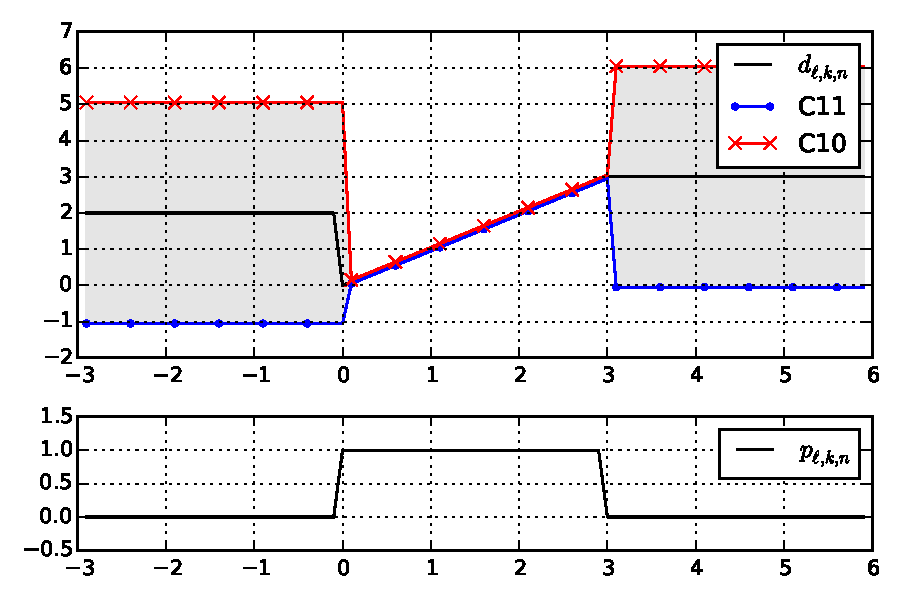
\includegraphics[width=0.45\textwidth,trim={0cm 0cm 0cm 0cm},clip]{phase_plot_fig_1.pdf}}
\subfigure[]{
\label{subfig:test2}
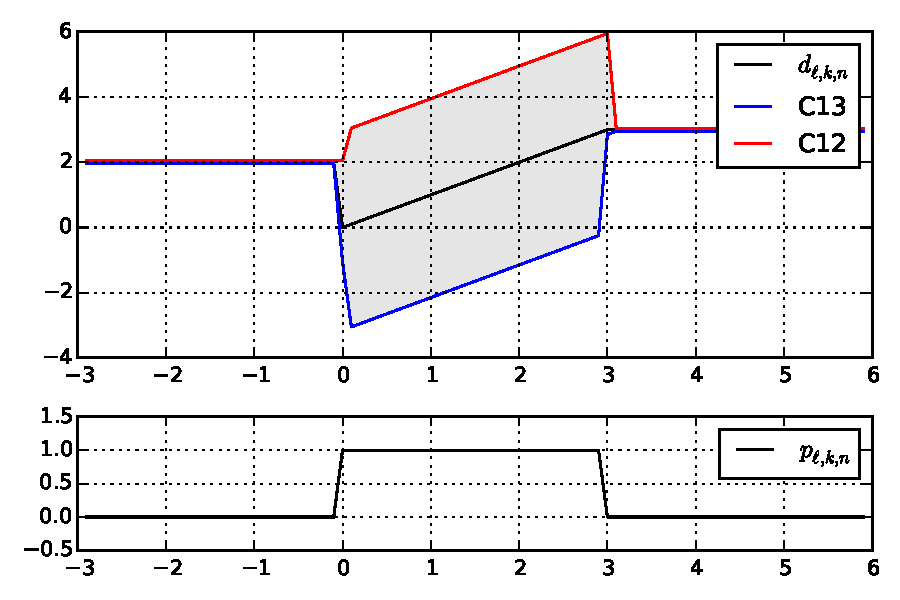
\includegraphics[width=0.45\textwidth,trim={0cm 0cm 0cm 0cm},clip]{phase_plot_fig_2.pdf}}
\subfigure[]{
\label{subfig:test3}
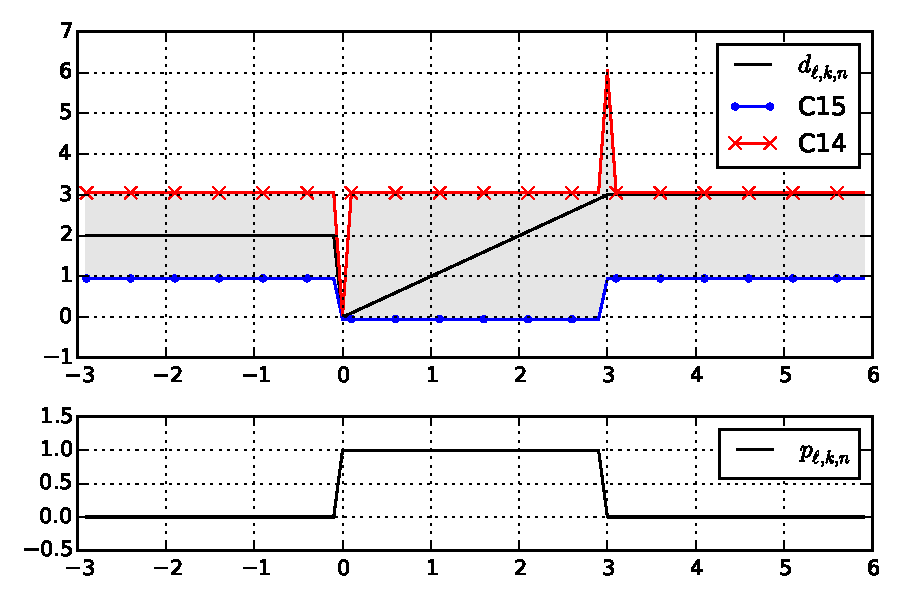
\includegraphics[width=0.45\textwidth,trim={0cm 0cm 0cm 0cm},clip]{phase_plot_fig_3.pdf}}
\subfigure[]{
\label{subfig:test4}
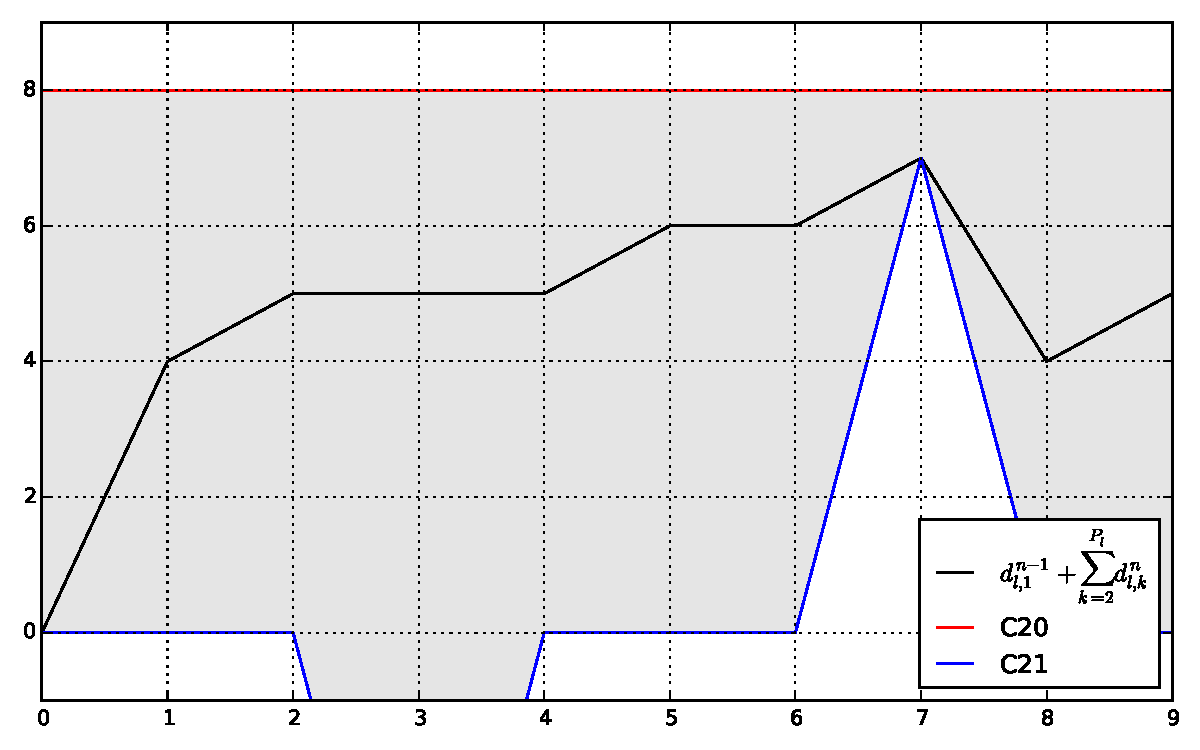
\includegraphics[width=0.45\textwidth,trim={0cm 0cm 0cm 0cm},clip]{phase_plot_fig_4.pdf}}
\caption{An example showing the phase and cycle time constraint envelopes. In
(a), (b) and (c), $\PTMIN{\ell}{k}=1$ and $\PTMAX{\ell}{k}=3$, the duration of
the previous activation was 2 and the duration of the current activation is 3.
In (d), the total cycle time is 7 with $\CTMIN{\ell}=7$, $\CTMAX{\ell}=8$}
\label{fig:phase_plots}
\end{figure*}

